\clearpage
\subsubsection{x86 + MSVC + \olly}
\myindex{\olly}
\myindex{x86!\Registers!\Flags}

Если попробовать этот пример в \olly, можно увидеть, как выставляются флаги.
Начнем с функции \TT{f\_unsigned()}, которая работает с беззнаковыми числами.

В целом в каждой функции \CMP исполняется три раза, но для одних и тех же аргументов, 
так что флаги все три раза будут одинаковы.

Результат первого сравнения:

\begin{figure}[H]
\centering
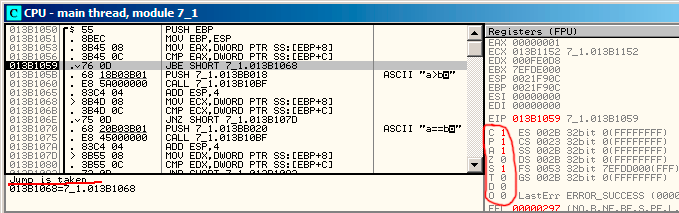
\includegraphics[scale=\FigScale]{patterns/07_jcc/simple/olly_unsigned1.png}
\caption{\olly: \TT{f\_unsigned()}: первый условный переход}
\label{fig:jcc_olly_unsigned_1}
\end{figure}

Итак, флаги: C=1, P=1, A=1, Z=0, S=1, T=0, D=0, O=0.
Для краткости, в \olly флаги называются только одной буквой.

\olly подсказывает, что первый переход (\JBE) сейчас сработает.  Действительно, если заглянуть в \cite{Intel}, 
прочитаем там, что \JBE срабатывает в случаях если CF=1 или ZF=1.
Условие здесь выполняется, так что переход срабатывает.

\clearpage
Следующий переход:

\begin{figure}[H]
\centering
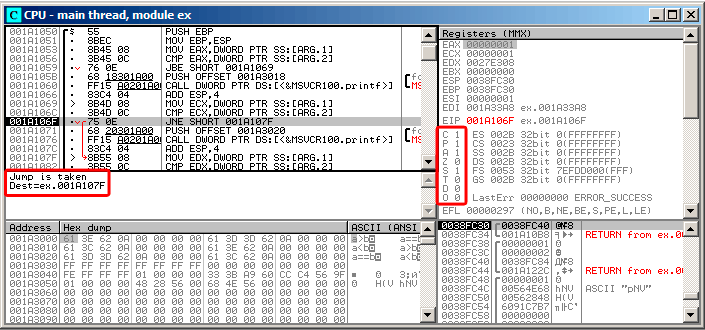
\includegraphics[scale=\FigScale]{patterns/07_jcc/simple/olly_unsigned2.png}
\caption{\olly: \TT{f\_unsigned()}: второй условный переход}
\label{fig:jcc_olly_unsigned_2}
\end{figure}

\olly подсказывает, что \JNZ сработает.
Действительно, \JNZ срабатывает если ZF=0 (zero flag).

\clearpage
Третий переход, \JNB:

\begin{figure}[H]
\centering
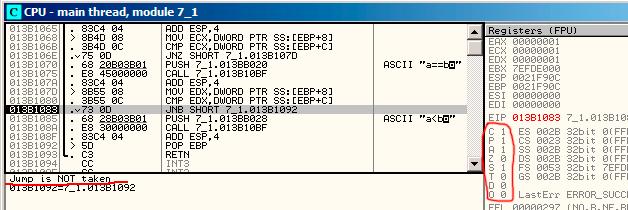
\includegraphics[scale=\FigScale]{patterns/07_jcc/simple/olly_unsigned3.png}
\caption{\olly: \TT{f\_unsigned()}: третий условный переход}
\label{fig:jcc_olly_unsigned_3}
\end{figure}

В \cite{Intel} мы можем найти, что \JNB срабатывает если CF=0 (carry flag).
В нашем случае это не так, переход не срабатывает, и исполняется третий по счету \printf.

\clearpage
Теперь можно попробовать в \olly функцию \TT{f\_signed()}, работающую с знаковыми величинами.
Флаги выставляются точно так же: C=1, P=1, A=1, Z=0, S=1, T=0, D=0, O=0.
Первый переход \JLE сработает:

\begin{figure}[H]
\centering
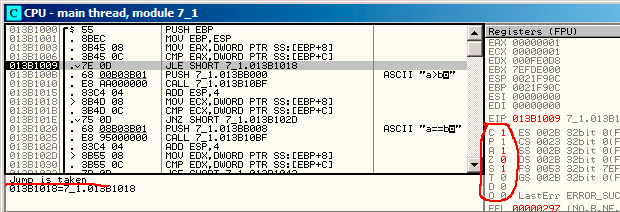
\includegraphics[scale=\FigScale]{patterns/07_jcc/simple/olly_signed1.png}
\caption{\olly: \TT{f\_signed()}: первый условный переход}
\label{fig:jcc_olly_signed_1}
\end{figure}

В \cite{Intel} мы можем прочитать, что эта инструкция срабатывает если ZF=1 \OrENRU SF$\neq$OF.
В нашем случае SF$\neq$OF, так что переход срабатывает.

\clearpage
Второй переход \JNZ сработает: он срабатывает если ZF=0 (zero flag):

\begin{figure}[H]
\centering
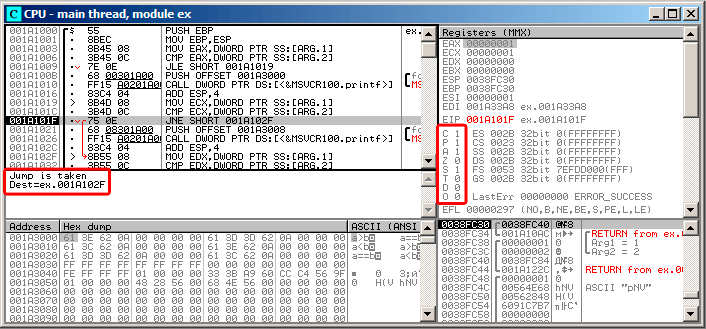
\includegraphics[scale=\FigScale]{patterns/07_jcc/simple/olly_signed2.png}
\caption{\olly: \TT{f\_signed()}: второй условный переход}
\label{fig:jcc_olly_signed_2}
\end{figure}

\clearpage
Третий переход \JGE не сработает, потому что он срабатывает, только если SF=OF, что в нашем случае не так:

\begin{figure}[H]
\centering
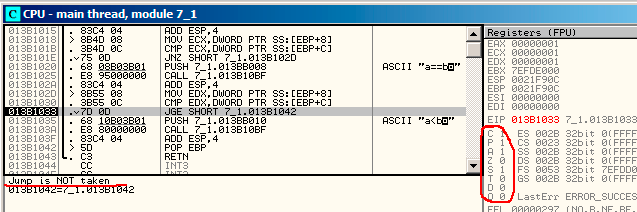
\includegraphics[scale=\FigScale]{patterns/07_jcc/simple/olly_signed3.png}
\caption{\olly: \TT{f\_signed()}: третий условный переход}
\label{fig:jcc_olly_signed_3}
\end{figure}
